% 样例 2：手拉手模型（part3/congruence/03 一图速记）
% 两个共顶点等腰三角形 △OAB 与 △OCD（顶角相等）
% 红色虚线 AC、BD 即"手拉手"两段（必相等）
\documentclass[tikz,border=4pt]{standalone}
\usepackage{ctex}
\usepackage{amsmath}
\usetikzlibrary{calc, decorations.markings}
\begin{document}
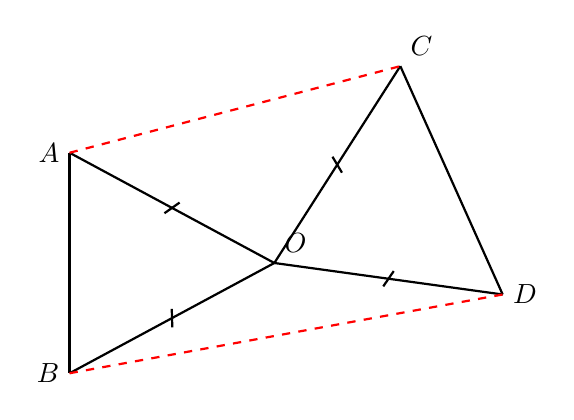
\begin{tikzpicture}[scale=1.0, thick,
  tick/.style={postaction={decorate, decoration={markings,
    mark=at position 0.5 with {\draw (-1.5pt,-3pt) -- (1.5pt,3pt);}}}}]

  \coordinate (O) at (0, 0);
  \coordinate (A) at (-2.6, 1.4);
  \coordinate (B) at (-2.6, -1.4);
  \coordinate (C) at (1.6, 2.5);
  \coordinate (D) at (2.9, -0.4);

  % 两个等腰三角形（腰用同一种 tick 标"等长"）
  \draw[tick] (O) -- (A);
  \draw[tick] (O) -- (B);
  \draw (A) -- (B);
  \draw[tick] (O) -- (C);
  \draw[tick] (O) -- (D);
  \draw (C) -- (D);

  % 手拉手两段（红色虚线）
  \draw[red, dashed] (A) -- (C);
  \draw[red, dashed] (B) -- (D);

  % 标签
  \node[above right] at (O) {$O$};
  \node[left]        at (A) {$A$};
  \node[left]        at (B) {$B$};
  \node[above right] at (C) {$C$};
  \node[right]       at (D) {$D$};
\end{tikzpicture}
\end{document}
